\begin{figure}[H]
    \centering
    \begin{subfigure}{0.1\textwidth} \raisebox{0.5\height}{\fbox{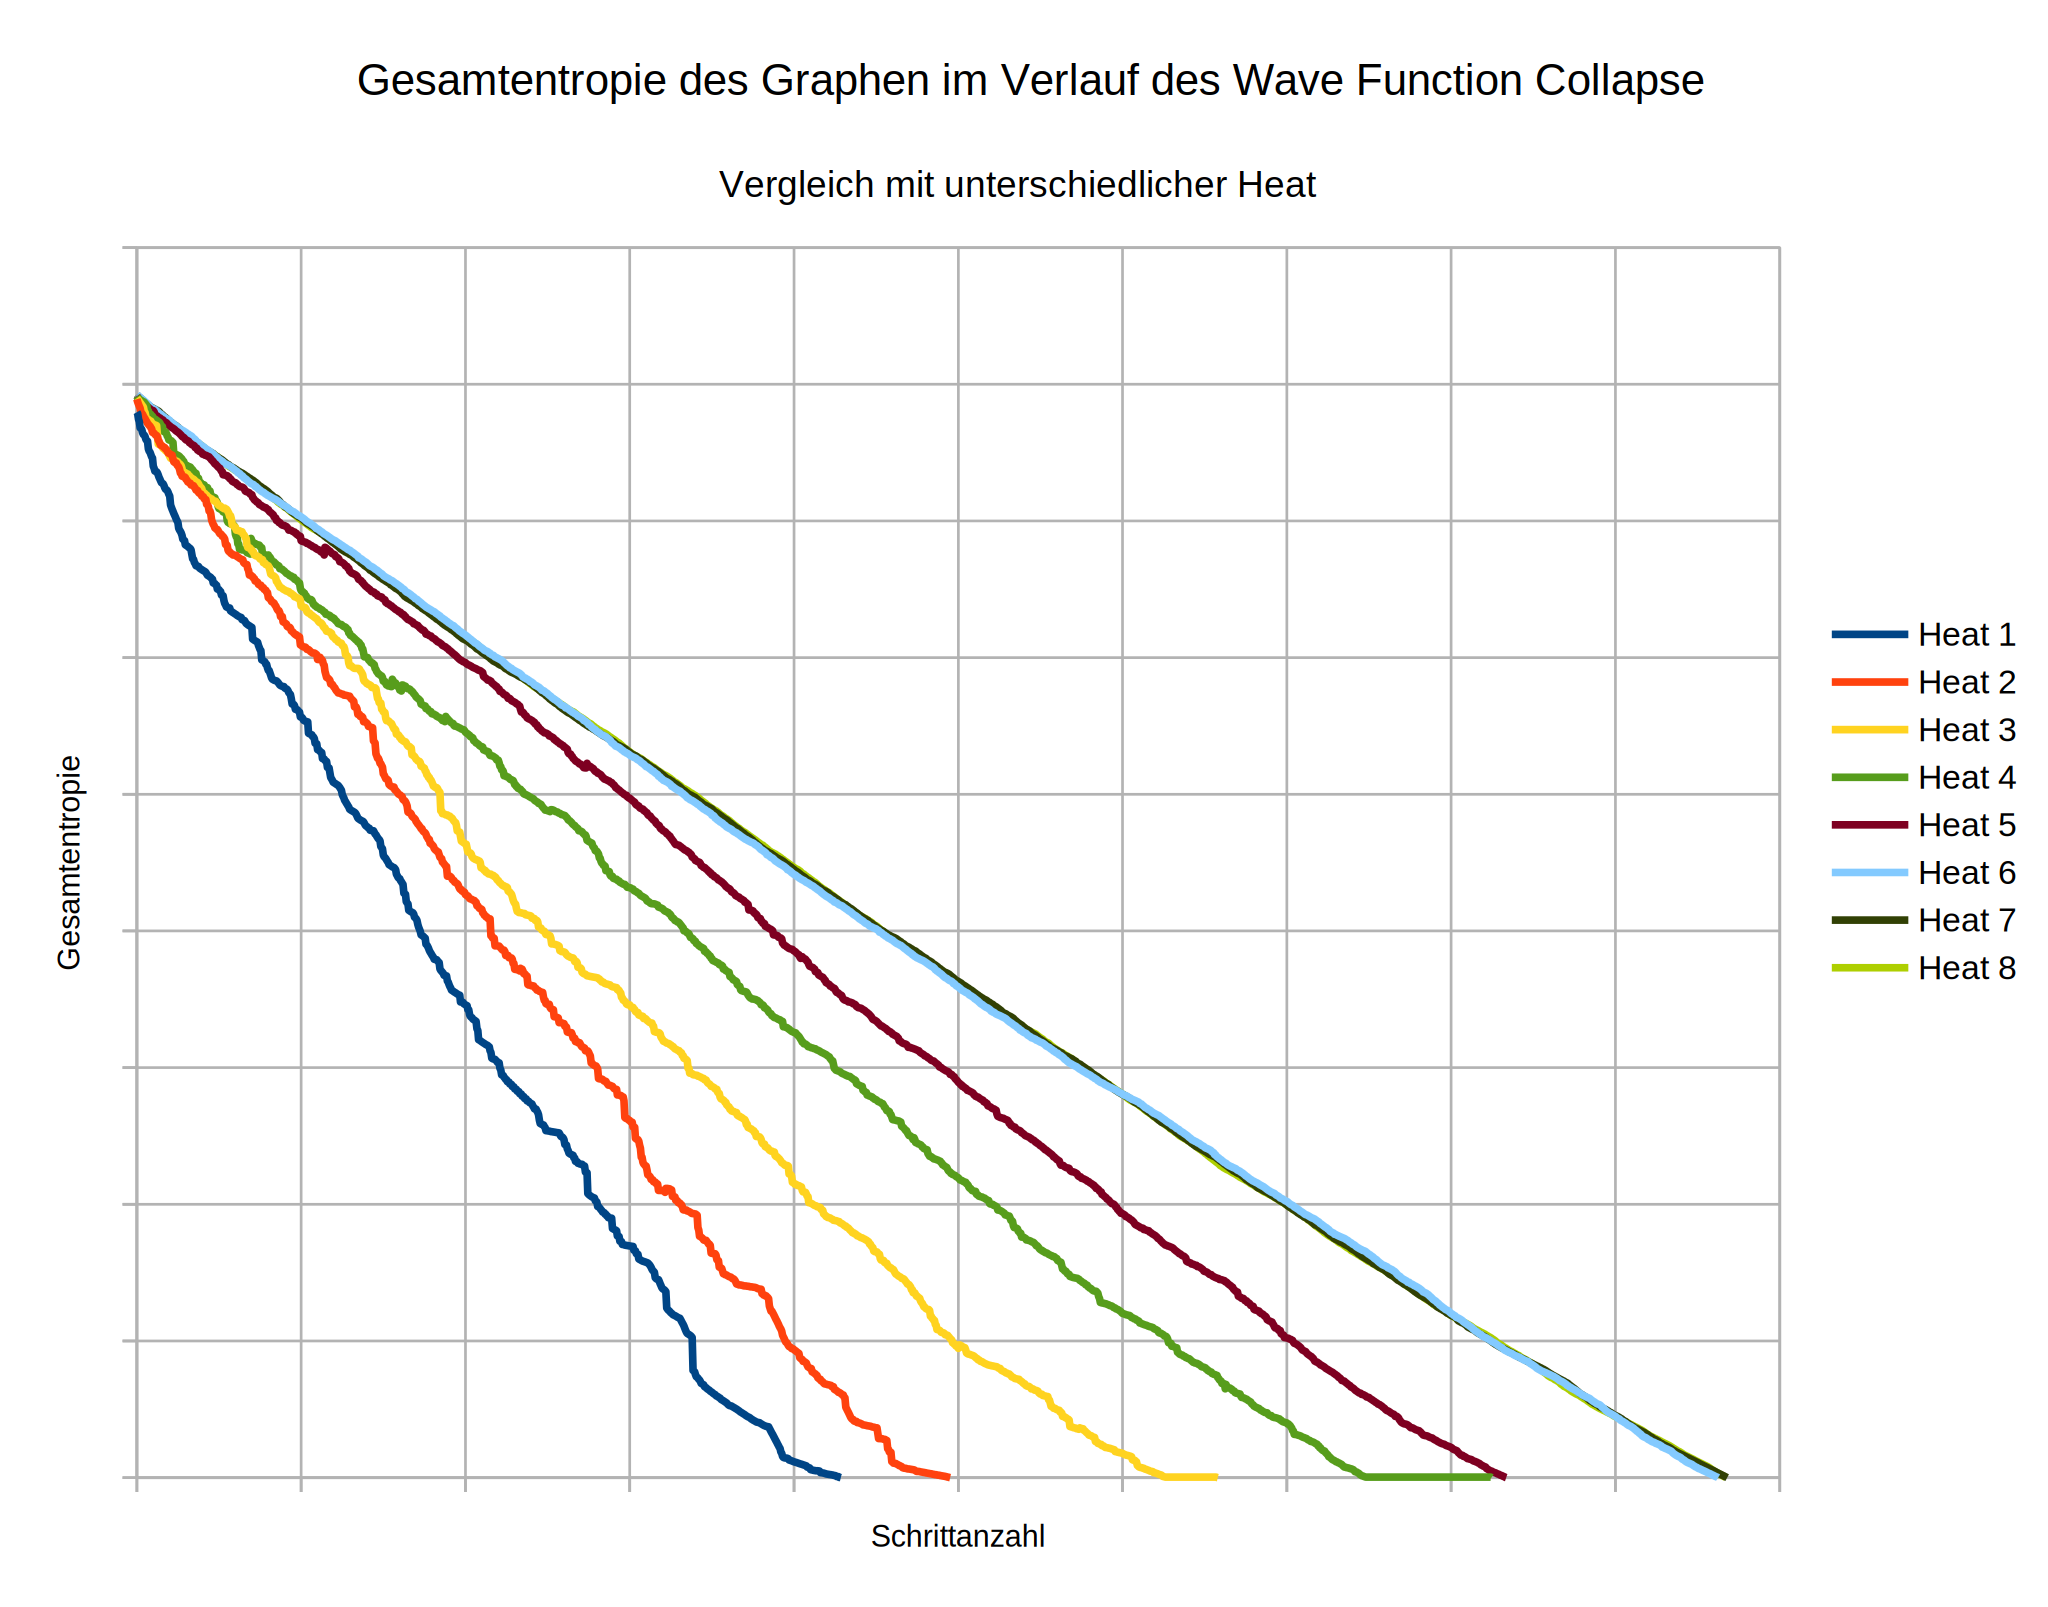
\includegraphics[width=\linewidth]{data/heat_rotation/1.png}}}  \caption{} \end{subfigure}
    \hspace{0.5em}
    \begin{subfigure}{0.2\textwidth}
        \includegraphics[width=\linewidth]{data/heat_rotation/2.png} \caption{0° Heat=1}
    \end{subfigure}
    \begin{subfigure}{0.2\textwidth}
        \includegraphics[width=\linewidth]{data/heat_rotation/3.png} \caption{22° Heat=1}
    \end{subfigure}
    \begin{subfigure}{0.2\textwidth}
        \includegraphics[width=\linewidth]{data/heat_rotation/4.png} \caption{23° Heat=1}
    \end{subfigure}
    \begin{subfigure}{0.2\textwidth}
        \includegraphics[width=\linewidth]{data/heat_rotation/5.png} \caption{23° Heat=2}
    \end{subfigure}
    
    \caption{
        Heat als lokale Drehung
    }
    \label{fig:heat_rotation}
\end{figure}